	\documentclass[twoside]{article}
\usepackage{../../estilo-ejercicios}
\renewcommand{\baselinestretch}{1,4}
%--------------------------------------------------------
\begin{document}

\title{Ejercicios de Topología Algebraica}
\author{Javier Aguilar Martín}
\maketitle

\begin{ejercicio}{2.1.9}\
Calcular los grupos de homología del $\Delta$-complejo $X$ obtenido de $\Delta^n$ identificando todas las caras de la misma dimensión. Esto es, $X$ tiene un solo $k$-símplice para cada $k\leq n$. 

 

\end{ejercicio}
\begin{solucion}\
Es claro que $C_i(X)$ está generado por una sola célula $e^i$ para cada $0\leq i\leq n$, por lo que el complejo de cadenas es simplemente
\[
0\to \Z\xrightarrow{d_n}\Z\xrightarrow{d_{n-1}}\cdots \xrightarrow{d_2}\Z\xrightarrow{d_1}\Z\to 0
\]
Como $X$ es conexo, $H_0(X)=\Z$ y esto significa que $d_1=0$. Veamos qué ocurre para $i>0$. Sea $e^i$ la célula que genera $C_i(X)$. Como $e^1\cong\Delta^i$, en $S^{i-1}=\partial e^i$ podemos encontrar abiertos disjuntos homeomorfos a las caras de dimensión $i-1$ de $\Delta^i$, que se pegan a $e^i$ con la orientación inducida por el símplice. Entonces, la aplicación $S^{i-1}\to X^{i-1}/X^{i-2}=S^{i-1}$ envía cada abierto de los descritos anteriormente a toda la esfera salvo un punto $y\in S^{i-1}$. La preimagen de todo punto $x\neq y$ consiste en un conjunto finito formado por $\binom{i+1}{i}=i$ puntos (el número de caras de dimensión $i-1$ de $\Delta^i$). Además, la orientación que induce el símplice es alternante, por lo que los grados locales alternan de signo y el grado total es $\sum_{j=0}^i(-1)^j$. Esto implica que $d_i=0$ si $i$ es impar (en particular para $d_1$, tal como habíamos calculado) y $d_1$ es isomorfismo para $i$ par. En homología esto se traduce en que $H_i(X)=0$ para todo $i\neq 0,n$, siendo $H_n(X)=\Z$ si $n$ es impar y $H_n(X)=0$ si $n$ es par. En resumen:
\[
H_i(X)=\begin{cases}
0 & i\neq 0,n\lor i=n \text{ par}\\
\Z & c.c.
\end{cases}
\]
\end{solucion}

\newpage

\begin{ejercicio}{2.1.14}
Determinar si existe una sucesión exacta corta $$0\to\Z_4\to \Z_8\oplus\Z_2\to \Z_4\to 0.$$ Más generalmente, determinar qué grupos abelianos $A$ forman una sucesión exacta corta $0\to\Z_{p^m}\to A\to\Z_{p^n}\to 0$ con $p$ primo. ¿Y en el caso de las sucesiones exactas cortas $0\to\Z\to A\to\Z_n\to 0$?
\end{ejercicio}
\begin{solucion}
Llamamos respectivamente $i$ y $j$ a las aplicaciones de la hipotética sucesión exacta corta. Por ser $i$ inyectiva, $\Ima{i}\cong\Z_4$, por lo que del primer teorema de isomorfía y la exactitud obtendríamos que $\Z_8\oplus\Z_2/\Z_4\cong\Z_4$. Esto no contradice el teorema de Lagrange, ya que las cardinalidades coinciden, y de hecho, en caso de que exista un subgrupo isomorfo a $\Z_4$ de modo que el cociente sea también isomorfo a $\Z_4$, esto nos da una manera de definir $j$. Identificamos los elementos del cociente $\Z_8\oplus\Z_2/\Z_4$ con las clases de equivalencia $\{\overline{0}, \overline{1},\overline{2},\overline{3}\}$. Para todo $x\in\overline{n}$, definimos $j(x)=n\in\Z_4$. Esta aplicación es un homomorfismo de grupos porque se conserva la estructura de grupo del cociente, es claramente sobreyectiva y su núcleo son los elementos de la clase $\overline{0}$, que son justamente los elementos del subgrupo isomorfo a $\Z_4$, y por tanto coinciden con $\Ima{i}$. Así pues, consideramos el subgrupo de $\Z_8\oplus\Z_2$ generado por $(2,1)$. El grupo $\Z_8\oplus\Z_2/\gene{(2,1)}$ tiene la presentación como grupo abeliano $\gene{a,b\mid 8a=0,2b=0, 2a+b=0}$, de donde obtenemos que $4a=0$ multiplicando la tercera ecuación por 2, y  $2a=b$ entre las dos últimas, de donde deducimos que efectivamente este grupo es isomorfo a $\Z_4$ (también se podría hacer calculando la forma normal de Smith de la matriz de coeficientes). Así que basta definir $i(1)=(2,1)$ y $j$ tal como se ha explicado anteriormente.

En el caso más general, $0\to \Z_{p^m}\to A\to \Z_{p^n}\to 0$, como $A$ tiene un subgrupo cíclico $B\cong\Z_{p^m}$ y un cociente cíclico $A/B\cong\Z_{p^n}$, $A\cong\Z_r\oplus\Z_s$ para ciertos enteros $r$ y $s$, pues podemos tomar como generadores un generador de $B$ y un representante de un generador de $A/B$. Por el teorema de clasificación de grupos abelianos, se puede tomar $r|s$. Por el teorema de Lagrange, $p^mp^n=|B||A/B|=|A|= rs$. Esto nos da $r=p^i$, $s=p^{m+n-i}$ con $0\leq i\leq \min\{m,n\}$. Con esto obtenemos una condición necesaria para $A$, veamos que es suficiente. Sean $r=p^i$ y $s=p^{m+n-i}$, con $0\leq i\leq\min\{m,n\}$. Como $i\leq m$, hay un homomorfismo sobreyectivo $\alpha:\Z_{p^m}\to \Z_{p^i}$. Por otro lado, 
\[
m+n-i\geq m+n-\min\{m,n\}=\max\{m,n\}+\min\{m,n\}-\min\{m,n\}=\min\{m,n\}\geq m
\] 
luego existe un homomorfismo inyectivo $\beta:\Z_{p^m}\to\Z_{p^{m+n-i}}$. Como $\beta$ es inyectivo, también lo es $(\alpha,\beta):\Z_{p^m}\to \Z_{p^i}\oplus\Z_{p^{m+n-i}}$. El conúcleo de esta aplicación tiene orden $p^n$ por el teorema de Lagrange, luego bastaría probar que es cíclico para comprobar que encaja en la sucesión exacta corta. Para ello, basta definir $\alpha(1)=(1,0)$ y $\beta(1)=(0, p^{m-i})$, que fácilmente se ve que verifican las condiciones de sobreyectividad e inyectividad. Ahora, el conúcleo de $(\alpha,\beta)$ tendría como presentación abeliana $$\gene{a,b\mid ap^i=0, bp^{m+n-i}=0, \alpha(1)=a=0, \beta(1)=bp^{m-i}=0},$$ de donde se obtiene que es cíclico con al simplificarla eliminando $a$ y $bp^{m+n-i}=bp^{m-i}p^n$.


  

Por último, consideremos la sucesión exacta corta $0\to\Z\to A\to \Z_n\to 0$. Veamos que $A=\Z\oplus\Z_d$ con $d|n$ encaja en ella. Definimos $\psi:\Z\oplus\Z_d\to\Z_n$ como $\psi(x,y)=x+cy$, donde $n=cd$, que es claramente sobreyectiva. Es claro que $\ker\psi=\gene{(c,-1)}\cong\Z$, luego si definimos $\phi:\Z\to \Z\oplus\Z_d$ mediante $\phi(1)=(c,-1)$, que es inyectiva, obtenemos la exactitud. Veamos que de hecho este es el único grupo salvo isomorfismo que podemos colocar en el lugar de $A$.
    
    
Supongamos ahora que $A$ encaja en la sucesión exacta corta. Considermos entonces el siguiente morfismo de sucesiones exactas cortas
\[
\begin{tikzcd}
0\arrow[r] & \Z\arrow[r]\arrow[d, equals] &\Z\times\Z\arrow[r]\arrow[d] & \Z\arrow[r]\arrow[d] & 0\\
0\arrow[r] &  \Z\arrow[r] & A \arrow[r] & \Z_n\arrow[r] & 0
\end{tikzcd}
\]
donde $\Z\times\Z\to A$ es cualquier homomorfismo de grupos, que sabemos que existe porque $A$ es un $\Z$-módulo, y además podemos tomarlo de modo que los cuadrados conmuten: 
\begin{itemize}
\item para que el cuadrado izquierdo conmute, primero definimos $\Z\to\Z\times\Z$ como $1\mapsto (1,0)$, y después $(1,0)$ se envía a la imagen del 1 mediante $\Z\to A$.
\item para que conmute el cuadrado derecho, en primer lugar definimos $\Z\times\Z\to\Z$ como $(1,0)\mapsto 0$ y $(0,1)\mapsto 1$, de modo que $(a,b)\mapsto b\mod n\in\Z_n$. Como $A\to\Z_n$ es sobreyectiva, enviamos $(0,1)\in\Z\oplus\Z$ a la preimagen de $1\in\Z_n$.  
\end{itemize}
 El Snake Lemma nos da el diagrama conmutativo siguiente, donde denotamos $\Z\times\Z\xrightarrow{\phi} A$
\[
\begin{tikzcd}
            & 0\arrow[d] & 0\arrow[d]                  & 0\arrow[d] &\\
 0\arrow[r] & 0\arrow[r]\arrow[d] & \ker\phi\arrow[d] \arrow[r, "\cong"] & n\Z\cong\Z\arrow[r]\arrow[d] & 0\\
 0\arrow[r] & \Z\arrow[r]\arrow[d, equals] & \Z\oplus\Z \arrow[r]\arrow[d] & \Z \arrow[r]\arrow[d] & 0\\
 0\arrow[r] & \Z\arrow[r]\arrow[d] & A\arrow[r]\arrow[d] & \Z_n\arrow[r]\arrow[d] & 0\\
            &       0     &        0   &   0
\end{tikzcd}
\]
En este diagrama, los 0 que no nos da directamente el Snake Lemma surgen de completar a partir del isomorfismo $\ker\phi\cong\Z$ salvo $A\to 0$, que es consecuencia de la demostración del lema de los cinco al ser $\Z\to\Z$ isomorfismo y $\Z\to\Z_n$ sobreyectiva. La columna central es una sucesión exacta corta isomorfa a la siguiente
\[
0\to \Z\xrightarrow{(n,r)}\Z\oplus\Z\to A\to 0
\]
para algún $r$ entero. La matriz $\binom{n}{r}$ se puede reducir a $\binom{d}{0}$, donde $d=\gcd(n,r)$, lo que, usando la exactitud junto con el primer teorema de isomorfía, nos da $A\cong \Z\oplus\Z_d$.
\end{solucion}

\newpage

\begin{ejercicio}{2.2.3}
Sea $f:S^n\to S^n$ una aplicación de grado cero. Probar que existen puntos $x,y\in S^n$ con $f(x)=x$ y $f(y)=-y$. Usar esto para probar que si $F$ es un campo vectorial continuo en la bola unidad $D^n$ en $\R^n$ tal que $F(x)\neq 0$ para todo $x$, entonces existe un punto en $\partial D^n$ donde $F$ apunta radialmente hacia fuera y otro punto en $\partial D^n$ donde $F$ apunta radialmente hacia dentro.
\end{ejercicio}
\begin{solucion}
La aplicación $f$ tiene puntos fijos, pues de lo contrario tendría grado $(-1)^{n+1}$, así que existe $x\in S^n$ con $f(x)=x$. Si consideramos ahora la antipodal $a:S^n\to S^n$, $\deg(a\circ f)=0$, luego también tiene puntos fijos, esto es, existe $y\in S^n$ con $a(f(y))=y$, con lo que $f(y)=-y$. 

Dado un campo vectorial continuo $F$ sobre la bola unidad $D^n$ tal que $F(x)\neq 0$ para todo $x$, podemos considerar el vector $F(x)$ como vector en el origen y normalizarlo, de modo que nos da una aplicación continua que también denotaremos $F:D^n\to S^{n-1}$. En particular, podemos considerar la restricción $f=F|_{\partial D^n}:S^{n-1}\to S^{n-1}$, que como se extiende de forma continua a $D^n$, es homotópicamente nula y por tanto tiene grado 0. Podemos aplicar ahora el resultado probado antes, de modo que existen $x,y\in S^{n-1}$ tales que $f(x)=x$ y $f(y)=-y$. El vector $F(x)$ apunta hacia fuera porque sigue el sentido del origen a $x$ y el vector $F(y)$ apunta hacia adentro porque sigue el sentido de $y$ a su antipodal.
\end{solucion}

\newpage

\begin{ejercicio}{2.2.10}
Sea $X$ el espacio cociente de $S^2$ bajo las identificaciónes $x\sim-x$ para $x$ en el ecuador $S^1$. Calcular los grupos homología $H_i(X)$. Hacer lo mismo para $S^3$ con puntos antipodales del ecuador $S^2\subset S^3$ identificados. 
\end{ejercicio}
\begin{solucion}
En el primer caso consideremos la estructura celular de $S^2$ obtenida con una 0-célula, una 1-célula y dos 2-células. El espacio cociente tiene la misma cantidad de células en cada dimensión, ya que se trata simplemente de dos copias de $\R P^2$ unidas por $\R P^1\cong S^1$, de modo que el complejo de cadenas tiene la forma
\[
0\to \Z\oplus\Z\xrightarrow{d_2}\Z\xrightarrow{d_1}\Z\to 0
\]
Como $X$ es conexo sabemos que $H_0(X)=\Z$ y por tanto $d_1=0$. Calculamos ahora $d_2$. Como el borde cada 2-célula se ``enrolla'' dos veces alreadedor de $S^1$, si denotamos $(a,b)$ a un elemento de $\Z\oplus\Z$, eligiendo adecuadamente los generadores obtenemos $d_2(a,b)=2a+2b$. Esto se puede ver también a partir de que el grado de la antipodal en $S^1$ es 1, con lo que las dos preimágenes de cada punto a las que da lugar el cociente tienen grado local 1, por lo que el grado total es 2. Así que $H_1(X)=\ker{d_1}/\Ima{d_2}\cong\Z_2$. Además, $H_2(X)=\ker{d_2}\cong\Z$. En definitiva,
\[
H_i(X)=\begin{cases}
\Z & i=0,2\\
\Z_2 & i=1\\
0 & c.c.
\end{cases}
\]

En el segundo caso, el $X$ es $\R P^2$ (que se puede obtener con una 0-célula, una 1-célula y una 2-célula) unido a dos 3-células con el borde identificado antipodalmente, es decir, $\R P^3$. Tenemos ahora el complejo de cadenas
\[
0\to\Z\oplus\Z\xrightarrow{d_3}\Z\xrightarrow{d_2}\Z\xrightarrow{d_1}\Z\to 0
\]
Igual que antes, $H_0(X)=\Z$ y $d_1=0$. Podemos calcular $d_2$ análogamente a como lo hicimos antes pero en este caso solo hay una célula, luego si denotamos $a$ al generador de $\Z$, $d_2(a)=2a$, de donde $H_1(X)\cong\Z_2$. Como $d_2$ es inyectiva, se tiene además que $H_2(X)=0$. Por último, $d_3=0$, pues la aplicación $S^2_{\beta}\to X^2/X^1=S^2_{\alpha}$ da para cada punto $x\in S^2_{\alpha}$ dos preimágenes, cada una en un hemisferio de $S^2_{\beta}$, en una el grado local es 1 porque la aplicación localemente es la identidad y en otra el grado es $-1$ porque la aplicación es localmente la antipodal, con lo que los grados locales se cancelan. Esto nos da $H_3(X)=\Z\oplus\Z$. En resumen,
\[
H_i(X)=\begin{cases}
\Z & i=0\\
\Z_2 & i=1\\
\Z\oplus\Z & i=3\\
0 & c.c.
\end{cases}
\]
\end{solucion}

\newpage


%\begin{ejercicio}{de las naranjas}
%Para el espacio $X$ de la imagen (donde las esferas se consideran huecas), calcular la homología local de todos sus puntos, hallar la mayor cantidad posible de subespacios $A\subseteq X$ tales que cualquier homeomorfismo $f:A\to X$ satisfaga $f(A)\subseteq A$, y estudiar si es posible asegurar que alguna potencia $f^n$ tenga puntos fijos, y en su caso cuántos. 
%
%\begin{figure}[h!]
%\centering
%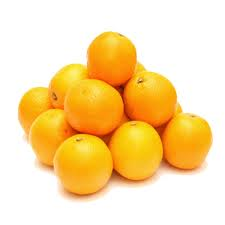
\includegraphics[scale=0.5]{naranjas}
%\end{figure}
%\end{ejercicio}
%\begin{solucion}
%Topológicamente distinguimos dos tipos de puntos en el espacio $X$: los puntos que tienen entornos homeomorfos a un disco abierto y los puntos donde las esferas se pegan, que tienen entornos homeomorfos a la unión puntual de dos discos abiertos. Sea $x\in X$ un punto del primer tipo y sea $U$ un entorno homeomorfo a un disco abierto. Entonces $U-x\simeq S^1$. La versión reducida de la sucesión exacta larga de homología relativa nos da $H_*(U,U-x)\cong \widetilde{H}_*(S^1)$, por lo que es 0 en todos los grados salvo $H_1(U,U-x)\cong\Z$. Sea ahora $x\in X$ con un entorno de $U$ de $x$ homeomorfo a la unión puntual de dos discos abiertos, de modo que $U-x\simeq S^1\sqcup S^1$. La sucesión exacta larga de homología relativa nos da $H_i(U,U-x)=0$ para $i>2$, $H_2(U,U-x)=\Z\oplus\Z$. Para los grados más bajos usamos la versión reducida, la cual nos da $H_1(U,U-x)=\Z$ y $H_0(U,U-x)=0$. Alternativamente podemos calcular la homología en grado 1 usando el ejercicio 2.1.16, de modo que $H_0(U,U-x)=0$ porque $U-x$ corta a la única componente conexa de de $U$. Como vemos, los puntos del primer tipo tienen homología local distinta a los del segundo, pues en el primer caso $H_2(U,U-x)=0$ y en el segundo $H_2(U,U-x)=\Z\oplus\Z$.
%
%\vspace{0.5cm}
%
%Vamos a la segunda parte del ejercicio. A los puntos del primer tipo los llamamos puntos de tipo I y a los del segundo tipo los llamamos puntos de tipo II. Lo primero que debemos notar es que cualquier homeomorfismo es en particular homeomorfismo local, y por tanto preserva la homología local, por lo que llevará puntos de tipo I en puntos de tipo I y puntos de tipo II en puntos de tipo II (todo esto en $A$, un punto de tipo $I$ en $A$ puede ser de tipo II en $X$). Vamos a suponer $A\neq\emptyset$, ya que en este caso trivialmente $f(A)=A$ y no hay puntos fijos para $f$ ni ninguna de sus potencias. Vamos a tratar primero el siguiente caso por orden de trivialidad, que sería $A=X$, donde también $f(A)=A$. Además, como hay una cantidad finitas de puntos de tipo II, digamos $k$ por ahorrarnos contar la cantidad exacta de este ejemplo, $f$ induce una permutación $\sigma_f\in S_k$, luego para $n=o(\sigma_f)$, $f^n$ tiene al menos $k$ puntos fijos. Para una potencia menor no es posible asegurar el mínimo de puntos fijos puesto que dependerá de la permutación en concreto, y tampoco podemos asegurar que no haya más porque podría haber puntos fijos en el resto de $X$. Una vez encontremos otro subespacio $A$ con $f(A)=A$, el mismo razonamiento será válido.
%
%%En primer lugar, $A$ no puede ser una esfera completa porque no tendría puntos de tipo II pero cualquier homeomorfismo la llevaría a una de las esfera, que sí tienen puntos de tipo II en $X$. Por otro lado, si $A$ está estrictamente contenido en una esfera menos los puntos de tipo II, siempre podemos tomar un homeomorfismo que deforme $A$ de modo que puntos que no estaban en $A$ aparezcan en la imagen. Así que $A$ debería contener como componentes conexas a algunas esferas menos sus puntos de tipo II. Observemos que las esferas del primer nivel tienen 3 puntos de tipo II salvo la central que tiene 4, las del segundo nivel tienen 5 puntos de tipo II y la esfera del tercer nivel tiene 4 puntos de tipo II. Por tanto, las componentes conexas de un nivel de $A$ van en ese mismo nivel, pues las de distintos niveles no son homeomorfas, pero las de un mismo nivel sí lo son. Si hubiera un nivel en el que $A$ tuviera alguna componente conxa pero no todas, entonces un homeomorfismo podría enviar una de las componentes conexas de $A$ en una de las de ese mismo nivel que no está en $A$. Por tanto, para cada nivel, $A$ debe o bien contenerlo por completo o bien no contener nada. Esto nos da todas las posibilidades para el caso en el que $A$ no contenga puntos de tipo II. 
%
%Si $A$ está estrictamente contenido en una de las esferas, podemos elegir un homeomorfismo que deforme $A$ de modo que puntos que no estaban en $A$ aparezcan en la imagen, así que $A$ debe contener esferas completas y solo esferas completas. De hecho debe contener más de una, porque si contuviera solo una, podría ser enviada con un homeomorfismo a cualquiera de las otra. De esto además se deduce que si $f(A)\subseteq A$, entonces se da de hecho la igualdad, ya que los homeomorfismos se reducen a permutaciones de esferas que mantienen la homología local y el razonamiento de los puntos fijos será valido para todos los subespacios fijos que encontremos.
%
%%Supongamos que $A\neq\emptyset$ EN ESTE PÁRRAFO LA CANTIDAD DE PUNTOS DE TIPO II ESTÁ MAL está contenido en el primer nivel de la pirámide. Entonces debe contener todas las esferas que dan al exterior, de lo contrario un homeomorfismo podría llevar una de las esferas de $A$ que dan al exterior a una de las que dan al exterior que no están en $A$. Esto es independiente de si $A$ contiene la esfera central porque cualesquiera combinaciones de la esfera central con $m$ de las que dan al exterior son homeomorfas entre sí. Además podemos comprobar que de hecho es necesario que en este caso $A$ contenga a la esfera central, de lo contrario podríamos elegir un homeomorfismo que llevara 3 esferas que hagan esquina en dos del segundo nivel y la del tercero. La esfera central tiene 4 puntos de tipo II, luego un homeomorfismo que no la lleve en sí misma solo podría llevarla a la esfera superior (en principio podría llevarla al segundo nivel, ocupando solo 4 de las 5 esferas adyacentes, pero se comprueba por inspección que esto no da lugar a un homeomorfismo) junto con las 4 esferas con las que está en contacto, que ocuparían el segundo nivel, pero esto no da posibilidad para que el resto de esferas de $A$ puedan ser mapeadas con un homeomorfismo, así que la esfera central debe quedar fija. 
%De ahora en adelante usaremos la siguiente notación para facilitar el enunciado y la comprensión: a la esfera superior la denotamos $S$, a la esfera central del nivel inferior la denotamos $C$, al resto de esferas del primer nivel las denotamos $E_i$, $i=1,\dots, 8$, siendo impares en las esquinas, y a las esferas del segundo nivel las denotamos $Z_j$, $j=1,\dots, 4$.
%
%
%Empecemos considerando subespacios que contentan a $S$. Es claro que añadiendo esferas solo del segundo nivel siempre podemos encontrar otros subespacios homeomorfos. Además, si incluimos alguna $Z_j$ en $A$, tendremos que incluirlas todas por simetría. Si además añadimos la esfera $C$, entonces ya no hay otro subespacio en el que haya dos esferas con 4 puntos de tipo II así que este verifica $f(A)=A$ para todo homeomorfismo. Además podríamos seguir añadiendo o bien las $E_{2k}$ o bien las $E_{2k+1}$ (o todas, pero eso nos daría $X$, que ya lo hemos estudiado). 
%
%Si no añadimos la esfera central, podemos o bien añadir las esferas $E_{2k}$ o bien las $E_{2k+1}$ (o todas). En cualquier otro caso podríamos encontrar un homeomorfismo que no deje invariante $A$ mediante rotaciones y simetrías. En los casos que hemos dado como válidos, $f(A)=A$ para cualquier homeomorfismo, ya que cualquier esfera que se enviara a una que no hayamos incluido tendría una cantidad distinta de puntos de tipo II. 
%
% Dentro de los subespacios que contienen a la esfera $S$ faltarían aquellos que no tienen ninguna esfera $Z_j$. Es claro que si $A$ no contiene la esfera $C$, entonces debe contener todas las exteriores y que este este sería un espacio invariante. Si $A$ contiene a $C$ hay más posibilidades. Una de ellas es que tenga todas las $E_i$, pero también podemos quedarnos solo con las $E_{2k}$ o solo con las $E_{2k+1}$, siendo esta última la única forma de elegir 6 esferas aisladas. 
% 
% Analizamos ahora los subespacio que no contienen a $S$. Si no $A$ no contiene tampoco ninguna $Z_j$, surgen los subespacios invariantes siguientes: $\bigcup_{i=0}^8E_i$ y $C\cup \bigcup_{k=0}^4E_{2k}$. En cualquier otro caso podríamos enviar homeomórficamente esferas de $A$ a un nivel superior o a esferas del nivel inferior que no estén en $A$. 
%
% 
% Si $A$ contiene alguna $Z_j$ pero no todas, por simetría podemos encontrar subespacios homeomorfos a $A$ que tienen esferas en este nivel que no están en $A$. Por tanto, nos centramos en los subespacios que contienen a todas las $Z_j$, que además deben contener esferas del nivel inferior, ya que hay más subespacios homeomorfos al espacio $\bigcup_{j=1}^4Z_j$. Si contiene además a $C$, tendrá que contener alguna esfera más porque de lo contrario podría enviarse $C\to S$. Por simetría, es necesario además que como mínimo sean o las cuatro $E_{2k}$ o las cuatro $E_{2k+1}$ (o todas las $E_i$). Si $A$ no contiene a $C$ en realidad también encontramos exactamente las mismas posibilidades, así que con esto hemos analizado todos los casos posibles. 
% 
%
% 
%\end{solucion}

\begin{ejercicio}{de las naranjas}
Para el espacio $X$ de la imagen (donde las esferas se consideran huecas), calcular la homología local de todos sus puntos, hallar la mayor cantidad posible de subespacios $A\subseteq X$ tales que cualquier homeomorfismo $f:X\to X$ satisfaga $f(A)\subseteq A$, y estudiar si es posible asegurar que alguna potencia $f^n$ tenga puntos fijos, y en su caso cuántos. 

\begin{figure}[h!]
\centering
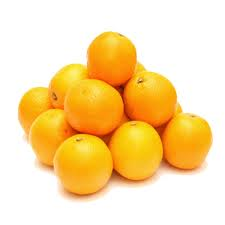
\includegraphics[scale=0.5]{naranjas}
\end{figure}
\end{ejercicio}
\begin{solucion}
Topológicamente distinguimos dos tipos de puntos en el espacio $X$: los puntos que tienen entornos homeomorfos a un disco abierto y los puntos donde las esferas se pegan, que tienen entornos homeomorfos a la unión puntual de dos discos abiertos. Sea $x\in X$ un punto del primer tipo y sea $U$ un entorno homeomorfo a un disco abierto. Entonces $U-x\simeq S^1$. La versión reducida de la sucesión exacta larga de homología relativa nos da $H_*(U,U-x)\cong \widetilde{H}_*(S^1)$, por lo que es 0 en todos los grados salvo $H_1(U,U-x)\cong\Z$. Sea ahora $x\in X$ con un entorno de $U$ de $x$ homeomorfo a la unión puntual de dos discos abiertos, de modo que $U-x\simeq S^1\sqcup S^1$. La sucesión exacta larga de homología relativa nos da $H_i(U,U-x)=0$ para $i>2$, $H_2(U,U-x)=\Z\oplus\Z$. Para los grados más bajos usamos la versión reducida, la cual nos da $H_1(U,U-x)=\Z$ y $H_0(U,U-x)=0$. Alternativamente podemos calcular la homología en grado 1 usando el ejercicio 2.1.16, de modo que $H_0(U,U-x)=0$ porque $U-x$ corta a la única componente conexa de de $U$. Como vemos, los puntos del primer tipo tienen homología local distinta a los del segundo, pues en el primer caso $H_2(U,U-x)=0$ y en el segundo $H_2(U,U-x)=\Z\oplus\Z$.

Vamos a la segunda parte del ejercicio. A los puntos del primer tipo los llamamos puntos de tipo I y a los del segundo tipo los llamamos puntos de tipo II. Lo primero que debemos notar es que cualquier homeomorfismo es en particular homeomorfismo local, y por tanto preserva la homología local, por lo que llevará puntos de tipo I en puntos de tipo I y puntos de tipo II en puntos de tipo II. 

Vamos a suponer $A\neq\emptyset$, ya que en este caso trivialmente $f(A)=A$ y no hay puntos fijos para $f$ ni ninguna de sus potencias. Vamos a tratar primero el siguiente caso por orden de trivialidad, que sería $A=X$, donde también $f(A)=A$. Además, como hay una cantidad finitas de puntos de tipo II, digamos $k$ por ahorrarnos contar la cantidad exacta de este ejemplo, $f$ induce una permutación $\sigma_f\in S_k$, luego para $n=o(\sigma_f)$, $f^n$ tiene al menos $k$ puntos fijos. Para una potencia menor, de momento no es posible asegurar el mínimo de puntos fijos puesto que dependerá de la permutación en concreto, y tampoco podemos asegurar que no haya más porque podría haber puntos fijos en el resto de $X$. Una vez encontremos otro subespacio $A$ con $f(A)\subseteq A$, el mismo razonamiento será válido para los puntos de tipo II de $A$. Así que el menor $n$ para el que podremos asegurar que $f^n$ tiene puntos fijos será el mínimo de los órdenes de las permutaciones que induzca $f$ en cada subespacio invariante. 

En adelante usaremos la siguiente notación: a la esfera superior la denotamos $S$, a la esfera central del nivel inferior la denotamos $C$, al resto de esferas del primer nivel las denotamos $E_i$, $i=1,\dots, 8$, siendo pares en las esquinas, y a las esferas del segundo nivel las denotamos $Z_j$, $j=1,\dots, 4$. 

Observamos que $C$ es la única esfera con 8 puntos de tipo II, por lo que debe quedarse fija por cualquier homeomorfismo, y de igual modo el complementario de los puntos de tipo II en $C$. En general, si un subconjunto de esferas permanece fijo, el subespacio resultante de eliminar los puntos de tipo II también lo estará por continuidad, no así cualquier subespacio $A$ estrictamente contenido en el complementario de los puntos de tipo II, ya que podemos encontrar homeomorfismos $f$ en en estas condiciones tales que $f(A)\not\subseteq A$. De igual modo, si $A$ contiene algún punto de tipo II pero no todos, este punto puede ser enviado mediante homeomorfismo a alguno de los no contenidos en $A$, así que $A$ debe tenerlos todos o ninguno. 

Observamos también que las esferas $E_{2k}$ son las únicas que tienen 3 puntos de tipo II, por lo que $\bigcup_{k=1}^4E_{2k}$ será un subespacio invariante. No lo será cualquier subespacio propio de este (salvo como ya comentábamos, este espacio menos los puntos de tipo II), puesto que una rotación intercambiaría las esferas entre sí. 

Las esferas $E_{2k-1}$ son las únicas que tienen 5 puntos de tipo II, así que por el mismo razonamiento $\bigcup_{k=1}^4E_{2k-1}$ es un subespacio invariante para todo homeomorfismo $f:X\to X$, y de nuevo ningún otro subespacio propio del complementario de los puntos de tipo II. 

Siguiendo el mismo razonamiento, como $S$ es la única esfera con 4 puntos de tipo II, debe ir en sí misma a través de todo homeomorfismo. 

Por último, las esferas $Z_j$ son las únicas que tienen 7 puntos de tipo II, lo que hace que el espacio $\bigcup_{j=1}^4Z_j$ sea un subespacio invariante por homeomorfismos. 

Con esto hemos estudiado todos los casos posibles de subespacios invariantes. Ahora podemos afinar un poco más para encontrar una potencia de $f$ que con seguridad tenga puntos fijos. El subespacio invariante con menos puntos de tipo II es $S$, que tiene 4, luego cualquier homeomorfismo $f:X\to X$ induce una permutación $\sigma_f\in S_4$. Como el máximo orden de un elemento de $S_4$ es 4, sabemos que $f^4$ tendrá al menos 4 puntos fijos. No podemos garantizar una potencia menor puesto que la permutación $(1,2,3,4)$ no fija ningún punto para una potencia menor. Pero podemos ir más allá en el conteo de puntos fijos. Al estar los 4 puntos de tipo II de $S$ fijos por $f^4$, cada una de las esferas $Z_j$ estarán fijas, y por tanto también los puntos $Z_j\cap Z_{j+1}$, que son otros 4 puntos. De aquí, también se mantienen fijos los 4 puntos de tipo II que surgen de la intersección $\bigcup_{j=1}^4Z_j\cap C$. El hecho de que las $Z_j$ estén fijas implica también que los puntos de tipo II de las $E_i$ estén fijos, con lo que finalmente deducimos que todos los puntos de tipo II permanecen fijos para $f^4$, sea cual sea el homeomorfismo $f$.


\end{solucion}
\end{document}
